\label{sec.GHDpredictions}\label{sec:ghd}
Le dispositif expérimental décrit ci-dessus peut être analysé théoriquement comme suit. Au cours de l'évolution temporelle, la frontière nette initiale du nuage devient plus lisse et les dérivées temporelles des quantités locales diminuent. Après un certain temps, après un lissage, on s'attend à ce que le gaz puisse être décrit localement par des états stationnaires.

Les états stationnaires du modèle de Lieb-Liniger sont complètement caractérisés par leur distribution de rapidité $\rho(\theta)$. Alternativement, ces états peuvent être caractérisés par le facteur d'occupation $\nu(\theta)$.% qui prend des valeurs entre 0 et 1, et qui est liée à la distribution de rapidité $\rho(\theta)$ par
%\begin{equation}
%\nu(\theta) = \frac{\rho(\theta)}{\rho_s(\theta)} \mbox{, \qquad où \qquad } \rho_s(\theta) =
%\frac{m}{2\pi \hbar} + \int \frac{d\theta'}{2\pi} \Delta(\theta-\theta') \rho(\theta') ,
%\end{equation}
%et $\Delta(\Theta) = \frac{2g}{\left(\frac{g^2}{\hbar} + \hbar \Theta^2\right)}$ est le "décalage de diffusion" dans le modèle de Lieb-Liniger. Les fonctions $\nu$ et $\rho$ sont en correspondance biunivoque, et dans ce qui suit, nous utilisons alternativement $\rho$ ou $\nu$. [Pour une introduction à ce formalisme, nous nous référons aux notes de cours \cite{doyon2020lecture} ou à la Section 1 de l'article de revue \cite{bouchoule_generalized_2022}.]

Puisque nous supposons une stationnarité locale, le système dans son ensemble est décrit par une distribution de rapidité dépendante du temps et de la position $\rho(x,\theta ; t )$, ou équivalemment par le facteur d'occupation dépendant du temps et de la position $\nu(x,\theta ; t)$. Ce dernier conduit à des calculs plus simples, tandis que le premier est particulièrement utile pour extraire la densité linéaire, qui est donnée par
\begin{equation}
    \label{eq:lineardensity}
	n(x;t) = \int d\theta \, \rho(x,\theta ; t ) .
\end{equation}

Les équations de GHD \cite{bertini_transport_2016,castro-alvaredo_emergent_2016} prédisent l'évolution temporelle de $\rho(x,\theta ; t)$, ou équivalemment de $\nu(x,\theta ; t)$. Lorsqu'elles sont écrites en termes du facteur d'occupation $\nu(x,\theta ; t )$, les équations de GHD prennent la forme d'une équation convective :
%\begin{subequations}
%\label{eq:GHD}
\begin{equation}
\label{eq:nu.cont}
\partial_t \nu  + v^{\rm{eff}}_{[\nu]} \partial_x \nu  = 0 ,
\end{equation}
avec la vitesse effective $v^{\rm{eff}}_{[\nu]}$ comme une fonctionnelle de la fonction d'ocumation (cf {??}).
Cette équation est un cas particulier particulier du problème de Rieman (??) avec initialement un facteur d'occumpation :
\begin{eqnarray}
	\label{eq:nu.cont.init}
	\nu(x, \theta ; t = 0 ) & = & \left \{\begin{array}{rcl} 0 & si & x<0 \\ \nu_0(\theta) & si & x>0 \end{array} \right. .
\end{eqnarray}

Soit \( \nu(x, \theta ; t) \) une solution de l’équation hydrodynamique (Eq.~\ref{eq:nu.cont}) vérifiant la condition initiale donnée en (Eq.~\ref{eq:nu.cont.init}). Considérons un changement d’échelle spatio-temporel : \( x \to x' = \alpha x \), \( t\to t' = \alpha t \). Alors, \( \nu(x', \theta, t') \) est également solution des équations hydrodynamiques avec les mêmes conditions initiales. En supposant l’unicité de la solution~\cite{???}, il en résulte que :

\begin{eqnarray}
\forall \alpha > 0 \colon \quad \nu(x, \theta; t) = \nu(\alpha x, \theta; \alpha t) = \nu\left(\frac{x}{\tau}, \theta; 1\right).
\end{eqnarray}
 Cette propriété de similarité est universelle pour les systèmes décrits par une dynamique hydrodynamique à l’échelle d’Euler.

%Autrement dit, \( \nu[\rho](x, \theta, \tau) \) ne dépend de \( x \) et \( \tau \) qu’à travers leur rapport \( x/\tau \). En particulier, le profil de densité au bord peut s’écrire sous la forme auto-similaire :

%\[
%n(x, \tau) = f[\rho]\left(\frac{x}{\tau}\right),
%\]
%
%où \( f[\rho] \) désigne une fonctionnelle de la distribution de rapidité \( \rho \).

%\begin{equation}
%v_{[\nu]}^{\rm{eff}}(\theta) = \theta - \int \Delta(\theta-\theta') \left( v^{\rm{eff}}_{[\nu]}(\theta) - v^{\rm{eff}}_{[\nu]}(\theta') \right) \rho(\theta') d\theta' .
%\end{equation}
%\end{subequations}
%Plus précisément, l'équation~(\ref{eq:GHD}a) est la forme à l'échelle d'Euler de la GHD, une équation sans diffusion valable aux grandes échelles. Des corrections diffuses, qui apparaissent sous forme d'un terme de type Navier-Stokes~\cite{de2018hydrodynamic,de2019diffusion,bastianello2020thermalization,de2022correlation}, ou même des corrections dispersives~\cite{de2023hydrodynamic}, ont également été étudiées théoriquement. Cependant, ces effets sont secondaires et n'ont pas été observés expérimentalement jusqu'à présent. Nous verrons plus bas que nos données expérimentales respectent le collage d'échelle attendu à l'échelle d'Euler (Fig.~\ref{fig:euler}), de sorte que ces effets semblent négligeables dans notre situation, du moins pour l'analyse des profils de frontière. Cela est également compatible avec une étude théorique récente dans le régime de faible interaction, qui a conclu que les effets diffusiques devraient être très faibles~\cite{moller2024identifying}. Par conséquent, dans cet article, nous ignorons la possibilité d'effets diffusiques secondaires (ainsi que tous les effets d'ordre supérieur) dans notre modélisation et nous nous en tenons à l'équation de GHD à l'échelle d'Euler ci-dessus.
\begin{figure}[!htb]
	\centering
	\includegraphics[width=\textwidth , page = 5 ]{Shema.pdf}
	\caption{
(a) À l'instant $t = 0^+$, immédiatement après le « quench bipartite » en $x = 0$, le facteur d'occupation est donné par $\nu(x, \theta ; t = 0^+) = \nu_0(\theta)$ pour $x > 0$ et est nul pour $x < 0$. Le bord initial représenté en tirets par l'ensemble des points $(x_b(s; t = 0^+) = 0,\ \theta(s; t = 0^+))$.
(b) Densité spatiale linéique $n(x)$ : en pointillés, $n(x; t = 0^-) = \int \rho(x, \theta; t = 0^-) \, \mathrm{d}\theta = n_0 = 56~\mu\mathrm{m}^{-1}$ juste avant le quench ; en ligne pleine, $n(x; t = 0^+) = n_0$ pour $x > 0$ et $0$ pour $x < 0$.
(c) À gauche de la coupure ($x < 0$) : en pointillés, $\nu(x, \theta ; t = 0^-) = \nu_0(\theta)$ ; en ligne pleine, $\nu(x, \theta ; t = 0^+) = 0$.
(d) À droite de la coupure ($x > 0$), le facteur d'occupation reste inchangé : $\nu(x, \theta ; t = 0^+) = \nu_0(\theta)$.
(e) À l'instant $t = 18~\mathrm{ms}$, après l'évolution balistique post-quench, le facteur d'occupation est donné par $\nu^\ast(x_b(s;t)/t, \theta) = \nu_0(\theta)$ pour $\theta < \theta_b(s;t)$, et nul pour $\theta > \theta_b(s;t)$, résolvant l'équation~(\ref{eq:nuetoile}), pour $t>0$. $\nu(x(s;t), \theta(s;t))(=\nu^\ast(x(s;t)/t, \theta(s;t)))$ est invarient de la déformation ie de $t>0$.  Le bord représenté en tirets par l'ensemble des points $(x_b(s; t)/t,\, \theta(s; t))$. Étant donné que la coupure initiale est en $x = 0$ et que l’évolution du bord est balistique, cette courbe résoud $v^{\mbox{\tiny eff}}_{[\nu^\ast(x(s; t)/t, \cdot) ]}(\theta(s; t)) = x(s; t)/t = v(s)$ (\ref{eq:nu.cont}).
(f) Densité spatiale  $n^\ast(x/t)$ en régime hydrodynamique (scaling).
(g) Pour les atomes à droite de la coupure : en pointillés, $\nu^\ast(x(s;t)/t, \theta) = \nu_0(\theta)$ ; en ligne pleine, $\nu^\ast(x_b(s;t)/t, \theta) = \nu_0(\theta)$ pour $\theta < \theta_b(s;t)$ et nul pour $\theta > \theta_b(s;t)$. Le raisonnement est similaire pour les atomes à gauche de la coupure.
}
	\label{fig:BiPart.coupure1}
	
\end{figure}

%\begin{figure}[hbt]
%    \centering
    %\includegraphics[width=0.7\textwidth]{Figures/figure_nustar.pdf}
%    \caption{Facteur d'occupation $\nu^* (v,\theta)$ résolvant l'équation (\ref{eq:nuetoile}) pour un ratio d'occupation initial $\nu_0 (\theta)$ dans la moitié droite du système correspondant à un équilibre thermique à température $T$. La ligne verte pointillée est la courbe $\theta^*(v)$, c'est-à-dire l'ensemble des points $(v,\theta)$ tels que $v^{\rm eff}_{[\nu^* (v,\cdot)]} (\theta) = v$. [Paramètres : 
%    $\gamma_0=mg/(n_0\hbar^2)=0.005$, $k_B T \hbar^2/(mg^2) = 365$, proches des paramètres expérimentaux des jeux de données ci-dessous.]}
%    \label{fig:nu_star}
%\end{figure}

Autrement dit, pour une bipartition initiale dont la discontinuité est située à $x=0$, la solution de \eqref{eq:GHD} est invariante le long des rayons de vitesse constante $x/t$~\cite{bertini_transport_2016,castro-alvaredo_emergent_2016}. En d'autres termes, l'équation \eqref{eq:GHD} implique que, pour cette classe d'états initiaux, la distribution du facteur d'occupation local et donc toutes les propriétés locales du gaz, dépendent de $x$ et $t$ uniquement à travers la quantité $v=x/t$. La solution de l'équation \eqref{eq:GHD} peut donc être écrite en utilisant le facteur d'occupation le long des rayons $\nu^*(v,\theta)$ tel que
\begin{equation}
	\label{eq:nuvsnuetoile}
    \nu(x,\theta ; t) = \nu^*( x/t,\theta).
\end{equation}

Pour la situation considérée dans cet article, où initialement un état de vide est situé pour $x < 0$ et un état de distribution du facteur d'occupation $\nu_0$ pour $x > 0$, la solution $\nu^*(v,\theta)$ est paramétrée par une rapidité de bord $\theta^*$ selon~\cite{bertini_transport_2016,castro-alvaredo_emergent_2016}
\begin{equation}
	\label{eq:nuetoile}
    \nu^*(v,\theta) = \left\{
    	\begin{array}{ccc}
    		\nu_0(\theta) & \text{si} & \theta < \theta^* \\
    		0 & \text{si} & \theta > \theta^* \\
   		\end{array}
    	\right. \quad \text{où} \quad  v^{\rm{eff}}_{[\nu^*(v,.)]}(\theta^*) = v.
\end{equation}
Cette équation peut être résolue numériquement pour toute distribution initiale donnée $\nu_0(\theta)$, voir la Fig.~\ref{fig:BiPart.coupure1} pour un exemple. Avec l'équation~\eqref{eq:nuvsnuetoile}, elle décrit entièrement le système à l'échelle d'Euler. Notez que, pour calculer la densité linéaire $n(x,t)$ afin de comparer avec les profils de densité expérimentaux, on utilise l'équation (\ref{eq:lineardensity}).

%\paragraph{Solution pour un système initialement dans l'état fondamental.}
%Pour illustrer le formalisme ci-dessus, explorons ses implications pour le cas spécial où la moitié droite du système est initialement dans l'état fondamental. Dans ce cas, le facteur d'occupation initial $\nu_0 (\theta)$ est une mer de Fermi : $\nu_0(\theta) = 1$ pour $|\theta| < \Delta\theta_0$, et $\nu_0(\theta) = 0$ sinon. Le rayon de Fermi $\Delta\theta_0$ dépend de la densité linéaire du gaz dans cette région, qui est constante. La distribution du facteur d'occupation se découpe ainsi en deux régions : pour $|\theta| > \Delta\theta_0$, $\nu_0(\theta) = 0$, et pour $|\theta| < \Delta\theta_0$, $\nu_0(\theta) = 1$. Au temps $t=0$, nous avons donc une discontinuité dans la distribution du facteur d'occupation à $\theta=\pm \Delta\theta_0$.

